%small gui blending in with iGraph,
%toggle labels,
%in-/decrease fontsize and amount of labels shown.

Im Gegensatz zu Änderungen der Magic Constants ist das GUI sicher. Es beachtet festgelegte Minimal- und Maximalwerte
und sorgt dafür, dass diese nicht unterschritten bzw. überschritten werden (sofern die Standardwerte in \texttt{consts.js} verwendet werden).

Die durch das GUI zu ändernden Parameter sind:
\begin{itemize}
    \item Label anzeigen (Toggle)
    \item Anzahl angezeigte Labels erhöhen
    \item Anzahl angezeigte Labels reduzieren
    \item Schriftgröße erhöhen
    \item Schriftgröße reduzieren
\end{itemize}

Weiterhin gilt zu sagen, dass für die Anzahl der gezeigten Labels im \hyperref[subsec:zoom]{Zoom Mode} weniger Labels angezeigt werden als sonst.
Um hier filigraner einstellen zu können, erfolgt das De-/Inkrementieren der Anzahl der gezeigten Labels in Einserschritten.
Für den normalen Modus werden mehrere Labels auf einmal hinzugefügt bzw. gelöscht.

Um Berechnungen für große Graphen zu reduzieren sind geringe Labelanzahl und Schriftgröße eines der besten Werkzeuge, sollten allerdings vom User eingestellt werden können - daher ein GUI.

\begin{figure}[H]
    \centering
    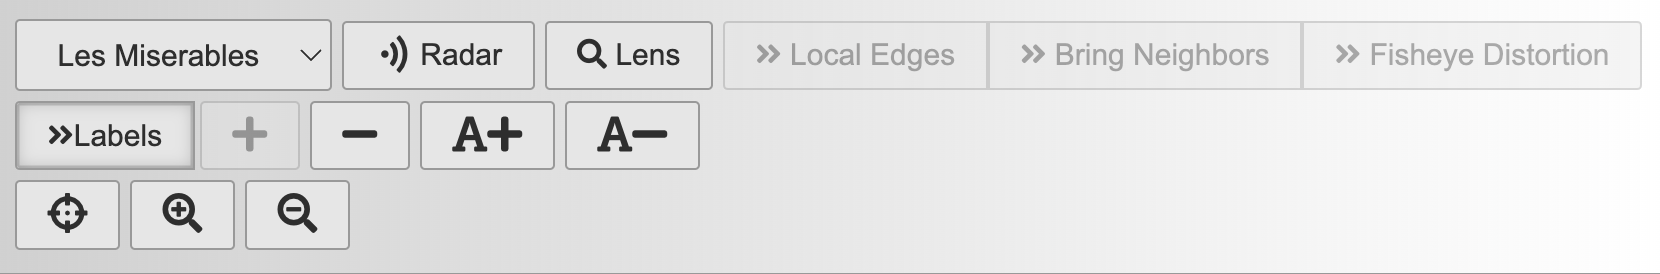
\includegraphics[width=\linewidth]{../img/gui}
    \caption{Simples GUI. Zweite Zeile ist verantwortlich für Labeling Einstellungen}
    \label{fig:gui}
\end{figure}
